\documentclass[a4paper,11pt]{article}
\usepackage[utf8]{inputenc}
\usepackage[ngerman]{babel}
\usepackage{geometry}
\usepackage{graphicx}
\usepackage{amsmath}
\usepackage{hyperref}
\usepackage{enumitem}

\geometry{a4paper, top=2cm, bottom=2cm, left=2cm, right=2cm}	

\usepackage{xcolor}
\definecolor{ohm_red}{RGB}{192,0,0}


\usepackage{fancyhdr}


\usepackage{titling}
\pretitle{\begin{flushleft}\LARGE}
\posttitle{\end{flushleft}}
\preauthor{\begin{flushleft}\large}
\postauthor{\end{flushleft}}

\setlength{\parindent}{0pt}



\pretitle{\begin{flushleft}\huge\textbf{\textcolor{ohm_red}}}
\posttitle{\end{flushleft}}

\pretitle{\begin{flushleft}\huge\textbf{\textcolor{ohm_red}}\rule{\linewidth}{0.4mm}\\}
\posttitle{\\\rule{\linewidth}{0.4mm}\end{flushleft}}
\title{\textcolor{ohm_red}{Einsatz eines Roboterhunds in der Such- und Erkundungsrobotik}}

\date{}


\usepackage{enumitem}
\setlist{nosep}

\pagestyle{fancy}
\renewcommand{\headrulewidth}{0pt}
\fancyhead[L]{
\includegraphics[height=2.0cm]{logo_autonohm.png}}
\fancyhead[R]{veröffentlicht am \today}


\usepackage{sidecap}

\sidecaptionvpos{figure}{c}


\begin{document}

\maketitle
\thispagestyle{fancy}

\vspace*{-3cm}
\begin{figure}[h!]
    \centering
    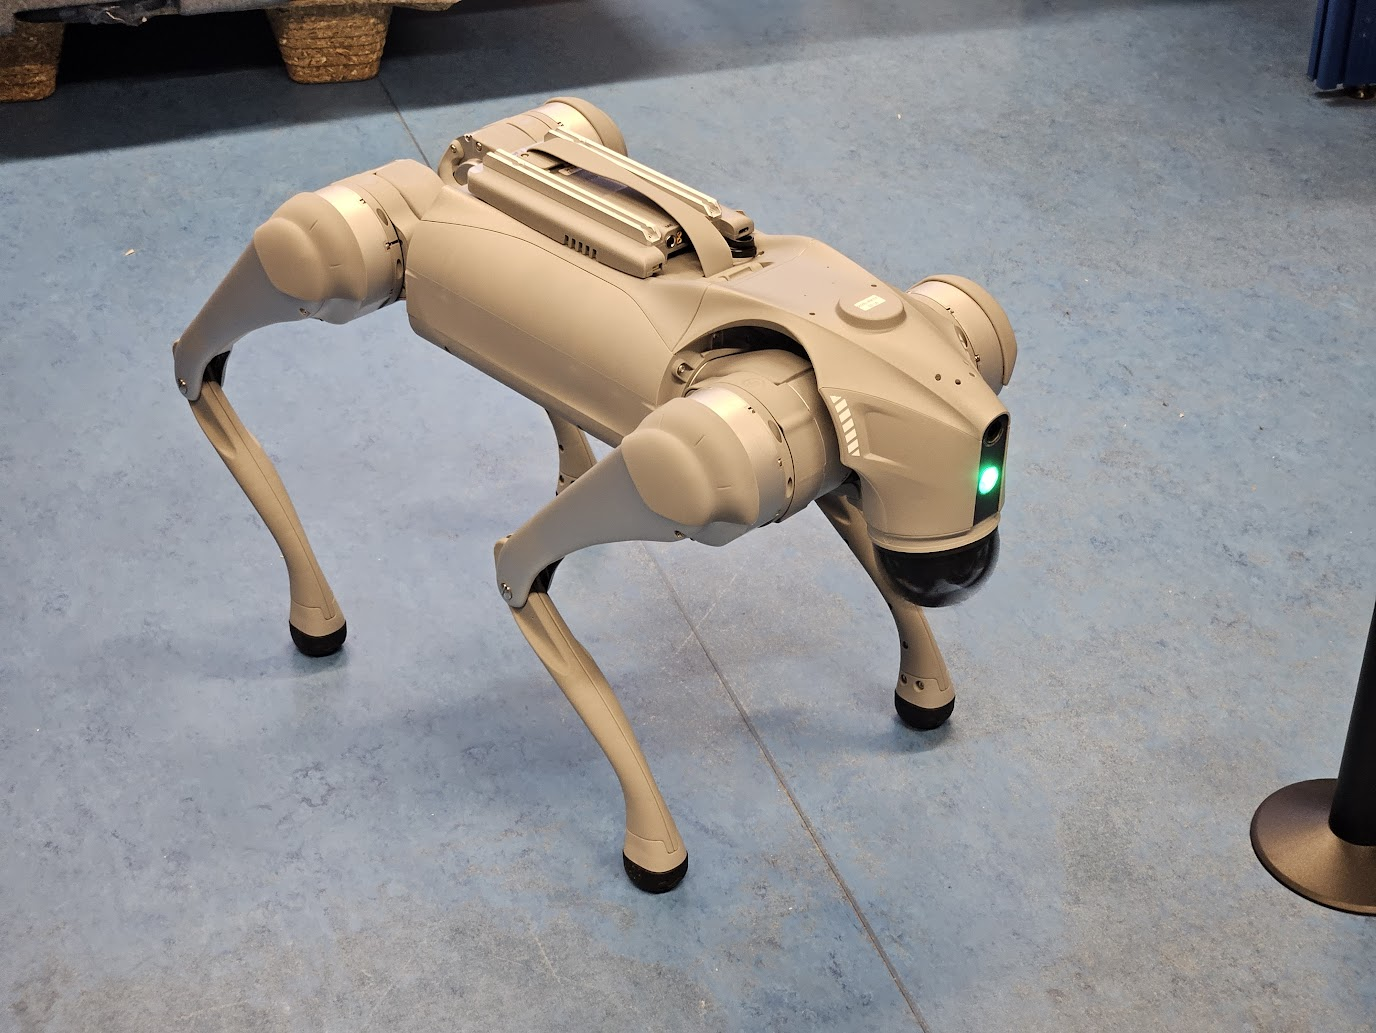
\includegraphics[height=4cm]{unitree.png}
    % \caption{Example Image}
    % \label{fig:example}
\end{figure}



Das Team \href{https://www.th-nuernberg.de/fakultaeten/efi/forschung/forschungsaktive-labore/mobile-robotik/}{AutonOHM} der Technischen Hochschule Nürnberg besitzt seit Kurzem einen Roboterhund vom Typ \href{https://www.youtube.com/watch?v=6zPvT0ig1VM}{Unitree Go2 Edu Plus}. Dieser Roboterhund ist ein vierbeiniger Roboter, der sich durch seine Agilität und Mobilität auszeichnet. Der Roboterhund ist mit einer Vielzahl von Sensoren ausgestattet, die es ermöglichen, die Umgebung zu erkunden und sich in dieser zu bewegen. 

Im Rahmen dieser Arbeit soll der Roboterhund in der \href{https://searchandrescuerobots.com/}{Such- und Erkundungsrobotik} eingesetzt werden. Hierbei soll der Roboterhund in der Lage sein, eine unbekannte Umgebung zu erkunden und dabei Hindernisse zu umfahren. Hierbei soll der Roboterhund autonom agieren und sich in der Umgebung zurechtfinden. Ziel ist die Integration bestehender open source Algorithmen aus der ROS-Community, um die Fähigkeiten des Roboterhundes zu erweitern. Weitere Informationen zu ROS finden Sie unter \href{https://docs.ros.org/en/foxy/index.html}{ROS-Dokumentation}. 

\section*{Arbeitspakete}
\begin{itemize}[leftmargin=0.5cm]
    \item Recherche von Softwarepaketen für die Such- und Erkundungsrobotik
    \item Integration der Softwarepakete in das bestehende ROS-System
    \item Auswahl von Softwarepaketen zur Kartierung der Umgebung
    \item Übertragung aller Sensordaten an eine Bedienerstation
    \item Implementierung von Algorithmen zur autonomen Navigation
    \item Test und Evaluation 
\end{itemize}

\section*{Voraussetzungen}
\begin{itemize}[leftmargin=0.5cm]
    \item Grundkenntnisse in ROS 
    \item Grundkenntnisse in einer höheren Programmiersprache (z.B. Python, C++)
    \item Grundkenntnisse in der Robotik
\end{itemize}

\vspace{0.5cm}
Das Thema kann nach Abstimmung als Bachelor- oder Masterarbeit bearbeitet werden, sowie als Projektarbeit. 


\vfill
\textcolor{ohm_red}{\rule{\linewidth}{0.4mm}}
\textbf{\textcolor{ohm_red}{Labor für mobile Robotik}} \\
\begin{tabular}{@{}ll}
\textbf{Betreuer:} & Prof. Dr. Christian Pfitzner \\
\textbf{E-Mail:}   & \href{mailto:christian.pfitzner@th-nuernberg.de}{christian.pfitzner@th-nuernberg.de} \\
\end{tabular}

\end{document}